\documentclass[conference]{IEEEtran}
\IEEEoverridecommandlockouts

\usepackage{cite}
\usepackage{amsmath,amssymb,amsfonts}
\usepackage{graphicx}
\usepackage{textcomp}
\usepackage{xcolor}
\usepackage{booktabs}
\usepackage{array}
\usepackage{tikz}
\usetikzlibrary{shapes.geometric,arrows.meta,positioning,fit,backgrounds,calc}
\usepackage{hyperref}
\hypersetup{colorlinks=false,pdfborder={0 0 0}}

\begin{document}

\title{Safety Communication Protocols in Industrial Automation:\\
A Comparative Study of PROFIsafe, FSoE, CIP Safety,\\
openSAFETY, and CC-Link IE Safety}

\author{
\IEEEauthorblockN{Sumon Boiddo}
\IEEEauthorblockA{Electronic Engineering\\
Hochschule Hamm-Lippstadt\\
Lippstadt, Germany\\
sumon.boiddo@stud.hshl.de}
\and
\IEEEauthorblockN{Nnaemeka Nnachi-Egwu}
\IEEEauthorblockA{Electronic Engineering\\
Hochschule Hamm-Lippstadt\\
Lippstadt, Germany\\
nnaemeka.nnachi-egwu@stud.hshl.de}
\and
\IEEEauthorblockN{Oluwasholape Daniel Oyemade}
\IEEEauthorblockA{Electronic Engineering\\
Hochschule Hamm-Lippstadt\\
Lippstadt, Germany\\
oluwasholape-daniel.oyemade@stud.hshl.de}
\and
\IEEEauthorblockN{Md Tawhidur Rahman Tuhin}
\IEEEauthorblockA{Electronic Engineering\\
Hochschule Hamm-Lippstadt\\
Lippstadt, Germany\\
md-tawhidur-rahman.tuhin@stud.hshl.de}
}

\maketitle

%% ── Abstract ─────────────────────────────────────────────────────────────────
\begin{abstract}
Standard IT networks offer best-effort delivery with no bounded latency
guarantee---a fundamental incompatibility with the demands of industrial
safety systems, where a single missed or delayed packet can result in a
fatal injury. This paper presents a comparative analysis of the five
dominant functional-safety communication protocols deployed over
Industrial Ethernet: PROFIsafe, Fail Safe over EtherCAT~(FSoE),
CIP Safety, openSAFETY, and CC-Link~IE Safety. All five are governed
by IEC~61784-3 and implement the Black Channel principle, which isolates
safety logic from the transport layer by embedding independent error
detection directly in each safety payload. The protocols are analysed
across six dimensions: frame architecture, cyclic redundancy check
scheme, passivation mechanism, real-time performance (latency, jitter,
and minimum cycle time), third-party certification pathway under
IEC~61508, and actual industry deployment across eight industrial sectors.
Findings confirm that all five reach SIL~3~/~PL~e and that no single
protocol is superior in every dimension. Differentiating factors include
cycle-time determinism, geographic ecosystem, device catalogue breadth,
and the cost and openness of the certification pathway.
Protocol-selection guidance is provided for each major sector.
\end{abstract}

\begin{IEEEkeywords}
Functional safety, IEC~61508, IEC~61784-3, PROFIsafe, FSoE, CIP~Safety,
openSAFETY, CC-Link~IE Safety, Black Channel, Industrial Ethernet, SIL
\end{IEEEkeywords}

%% ── I. Introduction ──────────────────────────────────────────────────────────
\section{Introduction}

Consider a straightforward question: would you use standard Wi-Fi to
transmit an emergency-stop command to a 200-tonne hydraulic press?
Instinct says no, and the engineering reason is precise. Standard Ethernet
and Wi-Fi are designed for best-effort delivery---they maximise average
throughput but make no guarantee that any individual frame will arrive
within a bounded time window. For most applications this is acceptable.
For a safety circuit, a single late or lost packet can mean a robot arm
strikes an operator, a press brake closes on a hand, or a conveyor
continues running during maintenance.

Functional safety is defined by IEC~61508 as the part of overall safety
that depends on the correct operation of electrical, electronic, and
programmable systems~\cite{IEC61508}. The framework does not ask how
often a hazard will occur; it asks how reliably the system responds
when one does. The key metric is the Probability of dangerous Failure
per Hour~(PFH), and machines that guard human operators must typically
meet Safety Integrity Level~3~(SIL~3), which requires PFH\,$<$\,$10^{-7}$/h.
IEC~62061~\cite{IEC62061} and ISO~13849~\cite{ISO13849} translate these
requirements into concrete design obligations---certified communication
links are mandatory for Category~3 / PL~d and above machine designs.

When legacy fieldbus systems gave way to Industrial Ethernet in the
early 2000s, the industry gained bandwidth, flexibility, and IT
compatibility, but lost the deterministic guarantees of dedicated
wiring~\cite{Neumann2007,MoyneTilbury2007}. Each major Industrial
Ethernet ecosystem---PROFINET, EtherCAT, EtherNet/IP, POWERLINK, and
CC-Link~IE---subsequently developed its own safety sublayer. All of them
independently arrived at the same architectural solution: treat the
transport as an untrusted channel and embed all necessary error
protection directly in the safety payload. IEC~61784-3~\cite{IEC617843},
first published in 2010 and significantly revised in 2021, formalised
this into the \emph{Black Channel} principle and established a unified
certification framework for all safety protocol families.

The resulting market is fragmented along regional and ecosystem lines in
a way that creates a practical challenge for industry. A Siemens SIMATIC
S7-1500F safety programmable logic controller ships on identical hardware
worldwide, yet runs PROFIsafe on European production lines and CIP~Safety
in North American facilities. The protocol is not determined by the
hardware manufacturer but chosen by the system integrator based on the
existing network infrastructure and regional supply chains. A safety
engineer who works across multiple sites must therefore be competent in
several protocols simultaneously.

This paper provides a structured comparative analysis of the five
protocols that together cover more than 95\% of certified safe nodes
currently deployed on Industrial Ethernet~\cite{IEC617843,SiemensSafety}.
Each is examined on its frame architecture, error-detection scheme,
passivation behaviour, performance characteristics, certification pathway,
and real-world deployment across major industrial sectors. The paper
is organised as follows: Section~II reviews the evolution of industrial
safety communication and the three channel architectures defined by
IEC~61784-3. Section~III describes and compares the architecture of each
protocol. Section~IV evaluates performance, certification, and industry
deployment. Section~V presents conclusions and protocol-selection guidance.

%% ── II. Background ───────────────────────────────────────────────────────────
\section{Background}

\subsection{Evolution of Industrial Safety Communication}

The history of industrial safety communication begins in the 1980s with
dedicated fieldbus systems. PROFIBUS~DP, DeviceNet, and CC-Link provided
deterministic, low-latency communication over proprietary physical layers;
safety was implemented through dedicated wiring, relay circuits, or
vendor-specific sublayers~\cite{Pigan2008}. During this period, CANopen
Safety~(CiA~304)~\cite{CiACanopen} introduced the concept of embedding
safety data within a standard frame on CAN-bus networks---a technique
later generalised into the Black Channel model. CANopen Safety remains
relevant today in medical devices and building automation, but its
reliance on CAN-bus speeds and topologies places it outside the scope
of this Industrial Ethernet comparison.

The shift to Industrial Ethernet in the early 2000s brought dramatic
performance improvements: gigabit speeds, standard RJ-45 cabling, and
compatibility with enterprise IT infrastructure~\cite{MoyneTilbury2007}.
However, standard Ethernet provides no timing guarantees, and each
Industrial Ethernet variant solved real-time requirements differently.
EtherCAT processes frames on the fly as they pass through each node;
PROFINET uses scheduled isochronous real-time~(IRT) slots; EtherNet/IP
relies on UDP-based cyclic messaging. Safety extensions followed between
2005 and 2012, one per ecosystem, all independently converging on the
same approach. IEC~61784-3 unified their certification requirements
under the Communication Profile Family~(CPF) model, assigning each
protocol a unique identifier~\cite{IEC617843}.

\subsection{Black, White, and Grey Channel Architectures}
\label{sec:channels}

IEC~61784-3 identifies three architectures for safety communication,
distinguished by the level of trust placed in the transport
layer~\cite{IEC617843}, as illustrated in Fig.~\ref{fig:channels}.

\begin{figure}[t]
\centering
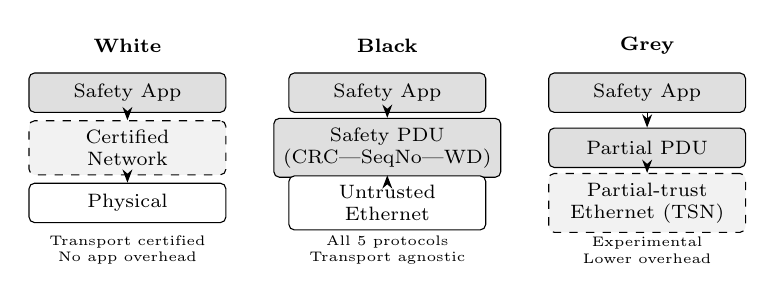
\begin{tikzpicture}[
  every node/.style={font=\scriptsize},
  box/.style={draw, rectangle, rounded corners=2pt,
              minimum width=2.5cm, minimum height=0.5cm, align=center},
  safe/.style={box, fill=gray!25},
  std/.style={box, fill=white},
  cert/.style={box, fill=gray!10, dashed},
  lbl/.style={font=\scriptsize\bfseries}
]

%% White Channel column
\node[lbl] (wt) at (0,4.2) {White};
\node[safe] (wa) at (0,3.6) {Safety App};
\node[cert] (wn) at (0,2.9) {Certified\\Network};
\node[std]  (wp) at (0,2.2) {Physical};
\draw[-Stealth] (wa)--(wn); \draw[-Stealth] (wn)--(wp);
\node[font=\tiny, align=center, text width=2.3cm] at (0,1.6)
    {Transport certified\\No app overhead};

%% Black Channel column
\node[lbl] (bt) at (3.3,4.2) {Black};
\node[safe] (ba) at (3.3,3.6) {Safety App};
\node[safe] (bp) at (3.3,2.9) {Safety PDU\\(CRC|SeqNo|WD)};
\node[std]  (be) at (3.3,2.2) {Untrusted\\Ethernet};
\draw[-Stealth] (ba)--(bp); \draw[-Stealth] (bp)--(be);
\node[font=\tiny, align=center, text width=2.3cm] at (3.3,1.6)
    {All 5 protocols\\Transport agnostic};

%% Grey Channel column
\node[lbl] (gt) at (6.6,4.2) {Grey};
\node[safe] (ga) at (6.6,3.6) {Safety App};
\node[safe] (gp) at (6.6,2.9) {Partial PDU};
\node[cert] (ge) at (6.6,2.2) {Partial-trust\\Ethernet (TSN)};
\draw[-Stealth] (ga)--(gp); \draw[-Stealth] (gp)--(ge);
\node[font=\tiny, align=center, text width=2.3cm] at (6.6,1.6)
    {Experimental\\Lower overhead};
\end{tikzpicture}
\caption{The three IEC~61784-3 channel architectures. White Channel
certifies the transport itself; Black Channel treats the transport as
fully untrusted; Grey Channel partially relies on transport-level
safety functions. All five protocols in this paper use Black Channel.}
\label{fig:channels}
\end{figure}

In a \emph{White Channel}, the transport is fully certified as safe.
The application layer requires no additional protective measures because
the network guarantees error-free, bounded delivery by design.
Historical examples include SafetyBUS~p and fieldbus-level AS-i Safety.
While conceptually simple, the White Channel demands certification of
the entire network infrastructure, making new deployments expensive,
inflexible, and largely obsolete.

In a \emph{Black Channel}, the transport is treated as completely
untrusted---equivalent to an adversarial or unreliable channel.
The safety protocol adds its own cyclic redundancy check~(CRC),
consecutive sequence number, connection identifier, and watchdog timer
directly to each payload frame. Together these measures detect all seven
transmission error classes defined by IEC~61784-3: corruption, unintended
repetition, incorrect sequence, loss, unacceptable delay, insertion, and
masquerading. No assumptions are made about the underlying network,
meaning the same safety sublayer can run unchanged over PROFINET, Wi-Fi,
or Modbus~TCP---a significant advantage for system integrators.

A \emph{Grey Channel} occupies intermediate ground: the transport provides
some safety functions, such as CRC or sequence numbering built into the
network protocol itself, but is not fully certified. The safety application
builds only the remaining required measures on top, reducing overhead
compared to the Black Channel. This model is currently being explored in
Time-Sensitive Networking~(TSN) profiles under IEC/IEEE~60802 but has not
yet reached the standardisation maturity of the Black Channel approach.

\subsection{Governing Standards}

The regulatory framework governing functional-safety communication operates
at three levels. IEC~61508~\cite{IEC61508} is the foundation, defining
SIL~1--4, PFH targets, and both hardware and software development lifecycle
requirements applicable to all safety-related systems. For machine safety
specifically, IEC~62061~\cite{IEC62061} defines SIL requirements for
Safety-Related Control Functions~(SRCF) and ISO~13849-1~\cite{ISO13849}
provides the parallel Performance Level~(PL~a--e) framework widely used
by European machine builders. IEC~61784-3~\cite{IEC617843} governs
communication directly, assigning each protocol a Communication Profile
Family identifier: CP~3/1 for PROFIsafe, CP~12/1 for FSoE, CP~2/1 for
CIP~Safety, CP~13/1 for openSAFETY, and CP~8/1 for CC-Link~IE Safety.
Installations in the process industry also reference IEC~61511, which
extends IEC~61508 to safety instrumented systems in oil, gas, and
chemical plant environments.

%% ── III. Protocol Architectures ──────────────────────────────────────────────
\section{Protocol Architectures}

\subsection{PROFIsafe (CP~3/1)}

PROFIsafe~\cite{IEC617843,SiemensSafety} is built on an F-Host/F-Device
model in which a safety PDU~(F-PDU) is inserted transparently into
standard PROFINET~IO data slots, requiring no modification to the
underlying PROFINET infrastructure. Each F-PDU carries a CRC-24 checksum
and an 8-bit F-Address combined with a monotonically increasing consecutive
number, which together provide sequence integrity and node identification.
The watchdog timeout is configured per-device through the F\_WD\_Time
parameter; expiry causes the F-Supervisor within the F-Host to passivate
all outputs of the affected F-Device. The engineering environment is TIA
Portal Safety, and the certified device catalogue exceeds 2\,000 products.

The F-PDU supports payloads of up to 123~bytes, accommodating complex
safety functions such as safe-torque-off~(STO) commands for multiple axes
in a single frame. PROFIsafe operates over both PROFINET~RT (software
real-time) and PROFINET~IRT (isochronous real-time); the latter provides
sub-microsecond jitter through hardware-scheduled slots.

With more than 35~million certified safe nodes globally, PROFIsafe holds
the largest installed base of any functional-safety protocol. It is the
dominant standard in European automotive assembly (Volkswagen Group,
BMW Group, Mercedes-Benz), heavy industry (ThyssenKrupp steel mills), and
process industries (BASF chemical plants, Shell refineries), where Siemens
SIMATIC infrastructure is widespread.

\subsection{Fail Safe over EtherCAT -- FSoE (CP~12/1)}

FSoE~\cite{IEC617843,ETG5100} uses a Master/Slave model. Each safety
frame consists of a Command Byte, User Data, Connection~ID, and CRC---
CRC-8 for payloads of up to two bytes, and CRC-16 for larger ones.
A 2-byte Safety Header Block~(SHB) carries the sequence number.
A critical design feature distinguishes FSoE from the other four protocols:
slave devices passivate autonomously when the watchdog expires, without
waiting for a reset command from the master. This eliminates one round-trip
from the reaction path and makes FSoE behaviour well-defined even in the
event of master failure. Combined with EtherCAT's distributed clock
synchronisation---which aligns all nodes to within~1\,ns---FSoE achieves
minimum cycle times of approximately 125\,\textmu{}s and jitter below
1\,\textmu{}s, the best figures in this comparison.
The safety overhead is the most compact at approximately 6~bytes, leaving
the bulk of the EtherCAT frame available for process data.

These characteristics make FSoE the protocol of choice for high-axis-count
motion control: FANUC robot cells in automotive tier-1 suppliers, TRUMPF
laser-cutting machines, and Beckhoff-equipped high-speed packaging lines
(Tetra~Pak, Bosch Packaging Technology) all run FSoE.

\subsection{CIP Safety (CP~2/1)}

CIP~Safety~\cite{IEC617843,ODVACIPSafety} maps safety connections over the
standard EtherNet/IP object model using Originator and Target roles.
Its most distinctive mechanism is a dual-packet format: the actual process
data and its bitwise complement are transmitted in the same frame, providing
a hardware-independent cross-check that is particularly robust against
systematic failures in the application layer. A Time Coordination Object
compensates for variable network propagation delays, an important provision
given that EtherNet/IP runs over unscheduled UDP. The Safety Supervisor
Object~(class~0x39) manages the connection state machine and passivation
sequence. The Target enters the safe state autonomously; no command
from the Originator is required.

The dual-packet design results in the highest protocol overhead among the
five at approximately 12~bytes, but it also enables the deepest integration
with existing EtherNet/IP infrastructure---safety and standard devices
share the same network without gateway hardware. CIP~Safety is the
de-facto standard in North American manufacturing: General Motors stamping
and body plants, Procter~\&~Gamble consumer goods lines, and Boeing
aerospace assembly all rely on it.

\subsection{openSAFETY (CP~13/1)}

openSAFETY~\cite{IEC617843,EPSGopenSAFETY} employs a frame-in-frame
design: the safety frame is embedded within the payload of a standard
POWERLINK or Modbus~TCP frame, and the transport layer processes it as
ordinary data. Each Safety Process Data Object~(SPDO) comprises two
independent sub-frames, each protected by its own CRC~(CRC-8 and CRC-16
respectively). Passivation is triggered only when both sub-frame checks
fail simultaneously, which significantly reduces nuisance trips caused by
transient single-bit errors---a practical advantage in electrically noisy
factory environments.

openSAFETY is the only royalty-free, fully open specification among the
five. Any vendor may implement the stack and submit it for independent
third-party certification without licensing from a standards consortium,
lowering the market-entry barrier for new device manufacturers.
This openness has driven adoption among European OEM machine builders:
Engel injection-moulding machines, Krones beverage bottling and labelling
lines, and B\&R-equipped production cells across the European packaging and
printing industries all use openSAFETY.

\subsection{CC-Link IE Safety (CP~8/1)}

CC-Link~IE Safety~\cite{IEC617843,CLPASafety} maps a Safety Communication
Layer~(SCL) into the cyclic frame structure of CC-Link~IE Field.
Each safety frame carries a CCITT CRC-16 checksum and combines a
node address with a frame counter for sequencing and anti-replay
protection. Unlike the other four protocols, which support arbitrary
network topologies, CC-Link~IE Safety is constrained to ring and line
configurations. Passivation is managed centrally by a Mitsubishi
MELSEC~iQ-R safety PLC, which monitors all nodes and coordinates the
safe-state transition. The engineering environment is GX Works3.

Certified under JIS~B~9961 (internationally recognised), CC-Link~IE
Safety is effectively mandatory for Tier~1 and Tier~2 suppliers to
Japanese automotive OEMs. Toyota Motor Corporation assembly plants,
Denso automotive component manufacturing, and Panasonic electronics
production are representative deployments.

\subsection{Comparative Architecture}

Table~\ref{tab:arch} summarises the key parameters across all five
protocols. Note that all five use the Black Channel model; the protocols
differ in CRC polynomial, sequencing mechanism, maximum payload, and
overhead, but not in their fundamental approach to safety independence
from the transport layer.

\begin{table}[h]
\caption{Protocol Architecture Comparison \cite{IEC617843}}
\label{tab:arch}
\centering
\scriptsize
\setlength{\tabcolsep}{3pt}
\renewcommand{\arraystretch}{1.15}
\begin{tabular}{l|ccccc}
\toprule
\textbf{Feature} & \textbf{PROFIsafe} & \textbf{FSoE} & \textbf{CIP} &
\textbf{openSFTY} & \textbf{CC-Lnk} \\
\midrule
CPF              & 3/1    & 12/1     & 2/1        & 13/1       & 8/1 \\
Channel          & Black  & Black    & Black      & Black      & Black \\
Max payload (B)  & 123    & 126      & Variable   & 8~(SPDO)   & 8 \\
CRC              & 24-bit & 8/16-bit & S1~(16-b)  & 8+16-bit   & 16-bit \\
Safety OH (B)    & $\sim$4 & $\sim$6 & $\sim$12   & $\sim$11   & $\sim$6 \\
Topology         & Any    & Any      & Any        & Any        & Ring \\
Open spec.       & No     & No       & No         & Yes        & No \\
\bottomrule
\end{tabular}
\end{table}

%% ── IV. Evaluation ───────────────────────────────────────────────────────────
\section{Evaluation}

\subsection{Performance Metrics}

Four metrics characterise real-time safety communication performance.
\emph{Minimum cycle time} is the fastest interval at which safety data
can be refreshed end-to-end. \emph{Typical jitter} measures the
cycle-to-cycle variance in delivery time, which is decisive for
motion-control applications where positional errors accumulate with each
missed synchronisation window. \emph{Safety reaction time} is the
worst-case elapsed duration from hazard detection to safe-state
actuation; it is typically two to three times the cycle time because
the watchdog must expire over multiple missed cycles before triggering
passivation. \emph{PFH} is the Probability of dangerous Failure per
Hour~\cite{IEC61508}, the quantitative SIL metric.

Throughput is deliberately excluded from this comparison. For safety
protocols, effective data rate is the product of payload size and cycle
frequency; since both quantities are already captured by the cycle time
and overhead rows, raw throughput adds no discriminating information.
Furthermore, all five protocols operate over 100~Mbps or 1~Gbps Industrial
Ethernet infrastructure, meaning the channel itself is never the bottleneck.
The binding constraint in every safety application is timing, not bandwidth.

\subsection{Performance Results}

Table~\ref{tab:perf} presents performance data drawn from protocol
specifications and vendor documentation.

\begin{table}[h]
\caption{Performance Comparison}
\label{tab:perf}
\centering
\scriptsize
\setlength{\tabcolsep}{2.8pt}
\renewcommand{\arraystretch}{1.15}
\begin{tabular}{l|ccccc}
\toprule
\textbf{Metric} & \textbf{PROFIsafe} & \textbf{FSoE} & \textbf{CIP} &
\textbf{openSFTY} & \textbf{CC-Lnk} \\
\midrule
Min.\ cycle & $\sim$1\,ms & $\sim$125\,\textmu{}s & $\sim$1--10\,ms &
  $\sim$400\,\textmu{}s & $\sim$500\,\textmu{}s \\
Jitter   & $<$1\,\textmu{}s & $<$1\,\textmu{}s & $\sim$100\,\textmu{}s &
  $<$1\,\textmu{}s & $\sim$1\,\textmu{}s \\
Reaction & $\sim$4--8\,ms & $\sim$1--2\,ms & $\sim$8--20\,ms &
  $\sim$2--4\,ms & $\sim$4--6\,ms \\
Max SIL  & SIL~3 & SIL~3 & SIL~3 & SIL~3 & SIL~3 \\
PFH ceil.& $<10^{-8}$/h & $<10^{-8}$/h & $<10^{-8}$/h &
  $<10^{-8}$/h & $<10^{-8}$/h \\
\bottomrule
\multicolumn{6}{l}{\scriptsize Sources: \cite{ETG5100,SiemensSafety,RockwellGuardLogix,BRopenSAFETY,CLPASafety}}
\end{tabular}
\end{table}

FSoE achieves the lowest cycle time and jitter by a significant margin,
a direct consequence of EtherCAT's hardware-level distributed-clock
synchronisation and FSoE's autonomous slave passivation. openSAFETY
follows closely, benefiting from POWERLINK's isochronous scheduling.
PROFIsafe with PROFINET~IRT also achieves sub-microsecond jitter but
requires a managed switch infrastructure and IEEE~1588 time
synchronisation to do so. CIP~Safety over EtherNet/IP operates over
unscheduled UDP, which produces higher and more variable jitter;
this is the trade-off for its superior interoperability with standard
network equipment and its ability to share the same IP network with
non-safety devices. CC-Link~IE Safety occupies the middle ground,
with determinism comparable to PROFIsafe~IRT but constrained to
ring topologies. For applications where process safety times exceed
10\,ms---the majority of light-curtain and E-stop applications---all five
protocols provide adequate headroom; for synchronised servo control
requiring reaction times below 2\,ms, FSoE is the only viable choice
from this group.

\subsection{Certification and Reliability}

All five protocols require assessment by an accredited third-party
certification body---TÜV~SÜD, TÜV~Rheinland, SGS-TÜV, or equivalent---
under IEC~61508 Part~3~\cite{IEC61508}. Hardware certification encompasses
failure mode and effects analysis~(FMEA), diagnostic coverage~(DC)
analysis, common-cause failure~(CCF) evaluation, and verification that
hardware fault tolerance~(HFT) matches the target SIL. Software must
comply with the IEC~61508 Part~3 development lifecycle; MISRA~C is the
prevalent coding standard for embedded safety stacks.
Ongoing reliability obligations include achieving the rated mean time
between failures~(MTBF) and conducting periodic proof tests; SIL~3
installations typically specify proof-test intervals of one to twenty years
depending on the PFH of the specific device.

openSAFETY carries a practical advantage in this dimension: as the only
royalty-free open specification~\cite{EPSGopenSAFETY}, any manufacturer
may implement and independently certify the stack without paying licensing
fees to a standards consortium, reducing the market-entry cost for new
device vendors. The other four protocols require a licensing relationship
with their respective owning organisations. CC-Link~IE Safety presents
a different consideration: its certificates are issued under
JIS~B~9961~\cite{CLPASafety}, which is internationally recognised but
requires an additional administrative layer for non-Japanese customers
comparing it against IEC~61508 documentation.

\subsection{Industry Deployment}

Table~\ref{tab:deploy} maps the five protocols across eight major
industrial sectors, categorising adoption as Primary~(P), Common~(C),
or negligible~(-), with representative real-world users.

\begin{table}[h]
\caption{Industry Deployment by Sector}
\label{tab:deploy}
\centering
\scriptsize
\setlength{\tabcolsep}{2.5pt}
\renewcommand{\arraystretch}{1.2}
\begin{tabular}{l|ccccc}
\toprule
\textbf{Sector} & \textbf{PROFIsafe} & \textbf{FSoE} & \textbf{CIP} &
\textbf{openSFTY} & \textbf{CC-Lnk} \\
\midrule
Auto.\ EU     & \textbf{P} (VW, BMW)   & C              & C              & --             & -- \\
Auto.\ N.Am.  & C                      & --             & \textbf{P} (GM,Ford) & --       & -- \\
Auto.\ APAC   & C                      & C              & --             & --             & \textbf{P} (Toyota) \\
Process ind.  & \textbf{P} (BASF)      & --             & C              & --             & -- \\
Machine bldg. & \textbf{P}             & C              & --             & C (Engel)      & -- \\
Food \& Bev.  & C                      & C (Tetra Pak)  & C              & C              & -- \\
Packaging     & C                      & \textbf{P} (Bosch) & C          & \textbf{P} (Krones) & -- \\
Electronics   & C                      & \textbf{P}     & C              & --             & C (Panasonic) \\
\bottomrule
\multicolumn{6}{l}{\textbf{P}\,=\,Primary;\quad C\,=\,Common;\quad --\,=\,negligible}
\end{tabular}
\end{table}

The deployment data reinforce two conclusions. First, no protocol dominates
across all sectors: PROFIsafe leads in European automotive and process
industries, CIP~Safety leads in North America, and CC-Link~IE Safety
is paramount in the APAC automotive supply chain. Second, FSoE and
openSAFETY are less regionally constrained and more application-constrained:
FSoE is the natural choice wherever EtherCAT motion control is already
installed, while openSAFETY is favoured by machine builders seeking
vendor independence.

%% ── V. Conclusions ───────────────────────────────────────────────────────────
\section{Conclusions}

This paper has compared PROFIsafe, FSoE, CIP~Safety, openSAFETY, and
CC-Link~IE Safety across architecture, performance, certification, and
industrial deployment. The principal findings are as follows.

All five protocols achieve SIL~3~/~PL~e under IEC~61508 and IEC~62061;
the safety ceiling itself is not a basis for selection. The protocols
differ meaningfully in cycle-time performance: FSoE and openSAFETY achieve
sub-millisecond cycle times and sub-microsecond jitter, making them the
preferred choice for motion-control applications; CIP~Safety accepts higher
jitter in exchange for seamless integration with existing EtherNet/IP
infrastructure. PROFIsafe commands the largest installed base and the
broadest certified device ecosystem, particularly in Europe and the process
industries. openSAFETY is the only royalty-free open specification,
offering the lowest certification barrier for new vendors. CC-Link~IE
Safety is effectively mandatory in the Japanese and broader APAC automotive
supply chain.

The Black Channel architecture underpins all five protocols and represents
the mature engineering consensus for functional safety over standard
Industrial Ethernet. The White Channel is obsolete for new designs.
The Grey Channel---currently being developed within TSN profiles under
IEC/IEEE~60802---may reduce protocol overhead while maintaining SIL~3
assurance, but has not yet reached production standardisation.

For practitioners, three factors should drive protocol selection:
the transport already deployed at the target site, the regional device
ecosystem and supply-chain availability, and the required safety reaction
time. Engineers working globally must expect to encounter all five protocols
across different sites, even on identical hardware platforms. Future work
should investigate the impact of IEEE~802.1~TSN on worst-case latency
guarantees for Black Channel safety sublayers, and the potential of Grey
Channel architectures to reduce overhead without sacrificing SIL~3 assurance.

%% ── References ───────────────────────────────────────────────────────────────
\bibliographystyle{IEEEtran}
\bibliography{references}

\end{document}
